%!TEX program = xelatex
%!TEX root = ../all.tex

\chapter{Linear regression}

\section*{Linear Models and Basis Function Expansion}

The foundation of many statistical learning algorithms lies in the use of \alert{linear models}. At their core, these models assume that the target prediction can be expressed as a linear combination of the input features. This assumption, while seemingly restrictive, provides the basis for powerful and interpretable mathematical frameworks.

%\subsection*{The Structure of Linear Predictors}

In its simplest form, a linear model predicts an output by scaling each input feature $x_i$ by a weight $w_i$ and adding a constant offset. Mathematically, for a $d$-dimensional input vector $\x = (x_1, \ldots, x_d)^T$, the hypothesis function $h$ is defined as:
\begin{myequation}
h(\x; w_1, \ldots, w_d, b) = w_1x_1 + w_2x_2 + \ldots + w_dx_d + b
\end{myequation}
Here, the constant term $b$ is known as the \alert{bias}. Its role is crucial: it allows the model to make a non-zero prediction even when all input features are zero, effectively shifting the decision surface away from the origin.

To simplify the notation, we typically represent the weights as a vector $\w \in \Real^d$. The model can then be written compactly using a dot product:
\begin{myequation}
h(\x; \w, b) = \w^T\x + b = 
\left(
\begin{array}{cccc}
w_1 & w_2 & \cdots & w_d
\end{array}
\right)
\left(
     \begin{array}{c}
          x_1 \\
          x_2 \\
          \vdots \\
          x_d
     \end{array}
     \right) + b
\end{myequation}

\textit{Commentary on Linearity:} It is essential to observe that these models are linear in two distinct ways. First, they are linear with respect to the \textbf{features} $\x$, describing a flat hyperplane in the input space. Second, and more importantly for optimization purposes, they are linear with respect to the \textbf{parameters} $\w$ and $b$. Since learning a model involves treating parameters as variables to be minimized or maximized, this linearity ensures that the resulting objective functions (such as sum-of-squares error) often have a convex shape, making the global optimum easy to find.

\subsection*{Feature Engineering and Basis Functions}

While the basic linear model is restricted to linear relationships in the original input space, we can greatly expand its expressive power through \alert{feature engineering}. This is achieved by mapping the original input $\x \in \Real^d$ into a new, typically higher-dimensional space $\Real^m$ using a set of predefined \alert{basis functions} $\{\phi_1, \ldots, \phi_m\}$.

The transformation is defined as $\Vphi(\x) = (\phi_1(\x), \ldots, \phi_m(\x))^T$. By applying this mapping, we transform a prediction task that might be non-linear in $\Real^d$ into a task that is linear in $\Real^m$. The modified model structure becomes:
\begin{myequation}
h(\x; \w, b) = \sum_{j=1}^{m} w_j\phi_j(\x) + b
\end{myequation}

It is a vital point that applying basis functions \textit{does not change} the linearity of the model with respect to its parameters $\w$. We are still performing a linear combination; we have simply changed the "ingredients" of that combination.

\subsubsection*{Common Types of Basis Functions}

The choice of basis functions determines the type of patterns the model can recognize. We generally categorize them into global and local functions:

\begin{itemize}
\item \textbf{Polynomial Basis Functions (Global):} 
These are defined as $\phi_j(x) = x^j$. They are "global" because a change in a single weight $w_j$ affects the prediction across the entire range of the input $x$. While powerful, they can be unstable at the boundaries of the data.
\begin{myequation}
\phi_{j}(x) = x^{j}
\end{myequation}

\item \textbf{Gaussian Basis Functions (Local):}
These take the form of a bell curve. They are "local" because the function $\phi_j(x)$ is only significantly non-zero in a small region around its mean $\mu_j$.
\begin{myequation}
\phi_{j}(x) = \exp\left(-\frac{(x-\mu_{j})^{2}}{2s^{2}}\right)
\end{myequation}

\item \textbf{Sigmoid Basis Functions (Local):}
The sigmoid function $\sigma(\cdot)$ maps the input to a range between 0 and 1. It represents a "step-like" transition centered at $\mu_j$.
\begin{myequation}
\phi_{j}(x) = \sigma\left(\frac{x-\mu_{j}}{s}\right) = \frac{1}{1+e^{-\frac{x-\mu_{j}}{s}}}
\end{myequation}

\item \textbf{Hyperbolic Tangent Basis Functions (Local):}
Similar to the sigmoid but mapping to the range $[-1, 1]$, the $\tanh$ function is often used in neural networks and signal processing.
\begin{myequation}
\phi_{j}(x) = \tanh(x) = 2\sigma(x)-1 = \frac{1-e^{-\frac{x-\mu_{j}}{s}}}{1+e^{-\frac{x-\mu_{j}}{s}}}
\end{myequation}
\end{itemize}



\centerline{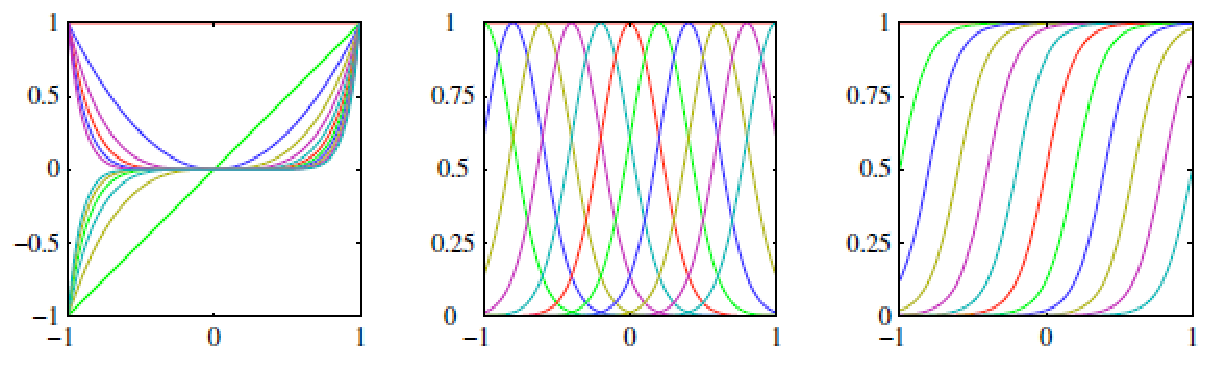
\includegraphics[width=12cm]{figure/fig11.pdf}}

%\subsection*{The Design Matrix}

In a practical training scenario, we deal with a dataset of $n$ observations, represented by the matrix $\X$:
\begin{myequation}
\X = \matrighe{\x_1}{\x_n} = \left(\begin{array}{cccc}
x_{11} & x_{12} & \cdots & x_{1d} \\
x_{21} & x_{22} & \cdots & x_{2d} \\
\vdots & \vdots & \ddots & \vdots \\
x_{n1} & x_{n2} & \cdots & x_{nd}
\end{array}\right)
\end{myequation}

When we apply our basis functions $\Vphi$ to every sample in the dataset, we construct the \alert{Design Matrix} $\VPhi$. Each row of this matrix corresponds to the transformed representation of a single data point, and each column represents the evaluation of a specific basis function across all samples:
\begin{myequation}
\VPhi = \left(\begin{array}{cccc}
\phi_{1}(\x_{1}) & \phi_{2}(\x_{1}) & \cdots & \phi_{m}(\x_{1}) \\
\phi_{1}(\x_{2}) & \phi_{2}(\x_{2}) & \cdots & \phi_{m}(\x_{2}) \\
\vdots & \vdots & \ddots & \vdots \\
\phi_{1}(\x_{n}) & \phi_{2}(\x_{n}) & \cdots & \phi_{m}(\x_{n})
\end{array}\right)
\end{myequation}

Moving forward, for the sake of simplicity, we will often refer to the original training set $(\X, \t)$. However, it is intended that all derivations and considerations apply equally to the transformed dataset $\VPhi$. Whether we are working in the original feature space or a mapped basis space, the underlying mechanics of linear optimization remain identical.



\begin{myexample}

Suppose we are provided with a set of $n$ observations involving two real-valued variables, $x$ (the input or independent variable) and $t$ (the target or dependent variable). This collection is represented as a set of pairs: 
\begin{myequation}
\{(x_1, t_1), (x_2, t_2), \dots, (x_n, t_n)\}
\end{myequation}
Our primary objective is \textbf{generalization}: we wish to exploit these specific observations to predict, for any new or unseen value $\tilde{x}$, the most likely corresponding value of the target variable $t$. 

In mathematical terms, we represent the training set as a pair of vectors:
\begin{itemize}
    \item $\x = (x_1, \ldots, x_n)^T$, representing the inputs.
    \item $\t = (t_1, \ldots, t_n)^T$, representing the observed targets.
\end{itemize}
These vectors are assumed to be related through an unknown deterministic rule, or function, which has been obscured by stochastic elements.

\begin{center}

\includegraphics[width=.3\linewidth]{Figure1-2a.pdf}
\end{center}


%\subsection*{The Generative Process and Noise}

To understand how to model this data, we must first make an assumption about how the data was generated. In this specific scenario, we assume that the "true" but hidden relationship between $x$ and $t$ is defined by a sine wave: $t = \sin(2\pi x)$. 

However, real-world data is rarely pristine. We assume the observations in our training set are corrupted by \alert{Gaussian noise}. This noise, denoted by $\varepsilon$, represents measurement errors or unobserved latent variables. We model this as a random variable with a mean of 0 and a specific variance $\sigma^2$, such that $\varepsilon \sim \mathcal{N}(\varepsilon; 0, \sigma^2)$. Consequently, each observed target $t_i$ is expressed as:
\begin{myequation}
t_i = \sin(2\pi x_i) + \varepsilon_i
\end{myequation}

Our goal is not to fit the noise, but to "see through" it to approximate the original deterministic function $t = \sin(2\pi x)$ as closely as possible, relying solely on the noisy evidence provided in the training set.

\begin{center}

\includegraphics[width=6cm]{Figure1-2.pdf}
\end{center}


%\subsection*{Polynomial Regression and Basis Functions}

One of the most versatile ways to approximate an unknown function is through \alert{polynomial regression}. In this approach, we choose to model the relationship using a polynomial of a fixed degree $m > 0$. The hypothesis function $h(x; \w, b)$ takes the form:
\begin{myequation}
h(x; \w, b) = w_1x + w_2x^2 + \ldots + w_mx^m + b = \sum_{j=1}^{m} w_j x^j + b
\end{myequation}
where $\w = (w_1, \ldots, w_m)^T$ represents the vector of coefficients and $b$ is the bias or intercept (effectively $w_0$). 

This model can be interpreted as a specific instance of a \textbf{linear model} operating in a transformed feature space. By defining a set $\Vphi$ of $m$ basis functions such that $\phi_j(x) = x^j$ for $j=1, \ldots, m$, we can rewrite the hypothesis as:
\begin{myequation}
h(x; \w, b) = \sum_{j=1}^m w_j \phi_j(x) + b
\end{myequation}

The choice of the degree $m$ is critical. A low value of $m$ (e.g., $m=1$, a straight line) might be too simple to capture the oscillations of the sine wave, leading to underfitting. Conversely, an excessively high value of $m$ might allow the polynomial to oscillate wildly to pass through every noisy data point, leading to overfitting.

The central challenge of the learning phase is to compute the optimal values for $\w$ and $b$ that minimize the discrepancy between our predictions $h(x_i)$ and the observed targets $t_i$.

\end{myexample}

\subsubsection*{Mathematical Optimization: Convexity and Global Minima}

To find the optimal parameters $\ow^*$, we must find the point where the gradient of $E(\ow)$ is zero. A critical advantage of the quadratic loss is that it is a \textbf{convex function}. Since the total error $E(\ow)$ is the sum of $n$ convex functions, $E(\ow)$ is itself convex.

In a convex landscape, any local minimum is guaranteed to be a \textbf{global minimum}. Furthermore, because the error function is quadratic, its derivative is linear. Solving for the point where this linear derivative equals zero yields a unique solution $\ow^*$, which defines our final predictor $h(\x;\ow^*)$.


To derive the optimal parameters analytically, we calculate the partial derivatives of the error function with respect to each weight and the bias:
\begin{myalign}
\frac{\partial E(\ow)}{\partial w_k}&=2\sum_{i=1}^nr_i(\ow)\frac{\partial}{\partial w_k}r_i(\ow)=2\sum_{i=1}^n\left(\sum_{j=1}^dw_jx_{ij}+b-t_i\right)x_{ik}\quad k=1,\ldots,d\\
\frac{\partial E(\ow)}{\partial b}&=2\sum_{i=1}^nr_i(\ow)\frac{\partial}{\partial b}r_i(\ow)=2\sum_{i=1}^n\left(\sum_{j=1}^dw_jx_{ij}+b-t_i\right)
\end{myalign}
This follows because $\frac{\partial}{\partial w_k}r_i(\ow) = x_{ik}$ (the value of the $k$-th feature for the $i$-th item) and $\frac{\partial}{\partial b}r_i(\ow) = 1$. Setting these $d+1$ equations to zero creates a linear system of equations that can be written in matrix form:
\begin{myequation}
\oX\overline{\w}=\t
\end{myequation}
where $\oX$ is the \textbf{augmented design matrix} including a leading column of ones to account for the bias:
\begin{myequation}
\oX = \left(\begin{array}{cccc}
1 & x_{11} & \cdots & x_{1d} \\
1 & x_{21} & \cdots & x_{2d} \\
\vdots & \vdots & \ddots & \vdots \\
1 & x_{n1} & \cdots & x_{nd}
\end{array}\right)
\end{myequation}
Assuming the matrix $\oX^T\oX$ is non-singular (which is generally true unless the data features are perfectly collinear), the unique solution is given by the \alert{normal equations}:
\begin{myequation}
\ow^*=(\oX^{T}\oX)^{-1}\oX^{T}\t
\end{myequation}

\subsection*{Numerical Optimization: Gradient Descent}

While the closed-form solution is mathematically elegant, it can be computationally expensive for very large datasets due to the matrix inversion. In such cases, we employ \alert{gradient descent}, an iterative numerical method that "walks" down the error surface toward the minimum.

\begin{enumerate}
\item \textbf{Initialization:} We start with an initial guess $\ow^{(0)}$, which results in an initial error $E(\ow^{(0)})$.
\item \textbf{Iterative Update:} At each step $s$, we modify the current parameters $\ow^{(s-1)}$ in the direction of the \textbf{steepest descent}. This direction is the negative of the gradient $\nabla E(\ow)$.
\item \textbf{Update Rule:} The parameters are updated using a \alert{learning rate} $\eta$:
\begin{myequation}
\ow^{(s)}:=\ow^{(s-1)}-\eta\nabla E(\ow)\Big|_{\ow^{(s-1)}}
\end{myequation}
Expanding this for the individual weights and the bias, we get:
\begin{myequation}
w_k^{(s)} := w_k^{(s-1)} - 2\eta \sum_{i=1}^nr_i(\ow^{(s-1)})x_{ik}, \quad b^{(s)} := b^{(s-1)} - 2\eta \sum_{i=1}^nr_i(\ow^{(s-1)})
\end{myequation}
\end{enumerate}



In matrix notation, the update looks like this:
\begin{myequation}
\ow^{(s)}:=\ow^{(s-1)}-2\eta \sum_{i=1}^nr_i(\ow^{(s-1)})\ox_i
\end{myequation}
where $\ox_i$ is the $i$-th row of the augmented design matrix. This update rule is highly intuitive: the change applied to the parameters is proportional to the residual $r_i$. If the model predicts an item perfectly, the residue is zero and no update occurs. If the error is large, the update is correspondingly large, pushing the model to correct its prediction for that specific data point.




\begin{myexample}
Consider the task of fitting a polynomial to a set of data points. This process involves applying a set of basis functions $\Vphi = (1, x, x^2, \ldots, x^M)$ to one-dimensional items. Here, $x^j$ represents the input $x$ raised to the $j$-th power, transforming our one-dimensional input into an $(M+1)$-dimensional space.

%\subsection*{The Process of Model Selection}

The choice of the polynomial degree $M$ is a fundamental example of \alert{model selection}. By assigning a specific value to $M$, we determine the internal representation of the items in our training set. This decision directly dictates the specific model we use because $M$ defines the number of coefficients in the weight vector $\w$ that must be estimated.

As we increase the complexity of the model by raising $M$, we provide the model with more degrees of freedom. This allows the polynomial curve to bend more flexibly, resulting in a better approximation of the training set items and a subsequent decrease in training error. However, this flexibility is a double-edged sword:
\begin{itemize}
    \item When $M$ is small (e.g., $M=0$ or $M=1$), the model might be too rigid to capture the underlying patterns, such as the oscillations of a sine wave.
    \item If the complexity increases to the point where $M+1 = n$ (where $n$ is the number of training samples), the model has enough parameters to pass exactly through every data point. This achieves a null training error, but it leads to the phenomenon of \alert{overfitting}.
\end{itemize}

\begin{figure}[ht]
\centering
    \begin{subfigure}[b]{.4\linewidth}
    \centering
    
\includegraphics[width=.6\linewidth]{Figure1-4a.pdf}
    \caption{$M=0$: Underfitting}
    \end{subfigure}
    \begin{subfigure}[b]{.4\linewidth}
    \centering
    
\includegraphics[width=.6\linewidth]{Figure1-4b.pdf}
    \caption{$M=1$: Linear fit}
    \end{subfigure}
\\
    \begin{subfigure}[b]{.4\linewidth}
    \centering
    
\includegraphics[width=.6\linewidth]{Figure1-4c.pdf}
    \caption{$M=3$: Balanced fit}
    \end{subfigure}
    \begin{subfigure}[b]{.4\linewidth}
    \centering
    
\includegraphics[width=.6\linewidth]{Figure1-4d.pdf}
    \caption{$M=9$: Overfitting}
    \end{subfigure}
\end{figure}

%\subsection*{The Generalization Challenge}

The core issue with overfitting is the failure of \textit{generalization}. While the hypothesis function $h(\x;\w,b)$ is derived exclusively from items in the training set, its true value lies in its ability to provide accurate predictions for new, unseen items across the whole domain.

If $h(\x;\w,b)$ is derived as a too much accurate depiction of the training set—essentially memorizing the noise rather than learning the signal—it results in an unsuitable generalization. In such cases, the model becomes "overly faithful" to the specific samples in the training set, losing the ability to predict the trend for items it has not encountered before.

%\subsection*{Evaluation of Generalization}

To observe this effect quantitatively in our example, we follow a specific experimental setup:
\begin{enumerate}
    \item Data Generation: We create a training set $\mathcal{T}_{train}$ of 1-dimensional items. These are generated by uniformly sampling $x$ in the interval $[0,1]$ and sampling noise $\varepsilon$ from a Gaussian distribution ${\cal N}(0,\sigma^2)$. The target is computed as $t = \sin(2\pi x) + \varepsilon$.
    \item Comparative Setup: We generate a separate test set $\mathcal{T}_{test}$ using the exact same probabilistic process. This set serves as our "unseen data."
    \item Measurement: For each degree $M$ under consideration:
    \begin{itemize}
        \item We derive the optimal weights $\w^*$ by minimizing the empirical risk on the training set $\overline{\mathcal{R}}_{\mathcal{T}_{train}}(\w)$.
        \item We then evaluate how these weights perform on the test set by computing the Root Mean Square (RMS) error:
        \begin{myequation}
        E_{RMS}(\w^*, \mathcal{T}_{test}) = \sqrt{\overline{\mathcal{R}}_{\mathcal{T}_{test}}(\w^*)} = 
        \sqrt{\frac{1}{|\mathcal{T}_{test}|}\sum_{(x_i,t_i)\in\mathcal{T}_{test}}\left(\sum_{j=0}^Mw^*_jx_{i}^j-t_i\right)^2}
        \end{myequation}
    \end{itemize}
\end{enumerate}



Note that since our basis set includes $\phi_0(x)=1$, the coefficient $w_0$ effectively acts as the bias $b$; thus, $b$ is implicitly handled within the weight vector $\w^*$. A lower value of $E_{RMS}(\w^*, \mathcal{T}_{test})$ indicates that the model has successfully generalized beyond the training data.

%\subsection*{Interpreting the Error Trends}

By plotting the $E_{RMS}$ with respect to the degree $M$ for both the training and test sets, we can identify the optimal complexity for our example.

\begin{center}

\includegraphics[width=.4\linewidth]{Figure1-5.pdf}
\end{center}

The resulting curves provide two crucial insights:
\begin{itemize}
    \item As $M$ increases, the error on the training set steadily decreases, eventually tending toward 0. This confirms that a more complex model can always "fit" a fixed set of points more closely.
    \item On the test set, the behavior is non-monotonic. Initially, the error decreases because the added complexity allows the model to capture the sinusoidal nature of the data. However, as $M$ continues to increase, the error begins to rise sharply. This occurs because the model becomes too dependent on the specific noise and distribution of the training set, leading to poor performance on any other data.
\end{itemize}
\end{myexample}

\section*{Regularization in Linear Models}

The phenomenon of overfitting is not solely a function of model complexity, but rather an interplay between the model's degrees of freedom and the quantity of information provided by the data. As we shall see, increasing the amount of evidence is one way to mitigate overfitting, while regularization provides a mathematical framework to control it directly when data is limited.

\subsection*{The Impact of Training Set Size}

A critical observation in machine learning is that for a fixed model complexity—for instance, a polynomial of a specific degree $M$—the tendency to overfit decreases as the dimension (size) of the training set increases. When more data points are available, the model is forced to satisfy a larger number of constraints, making it much harder for a complex curve to "wiggle" through every individual point while still capturing the true underlying signal.

\begin{figure}[ht]
\centering
    \begin{subfigure}[b]{.4\linewidth}
    \centering
  
\includegraphics[width=.7\linewidth]{Figure1-6a.pdf}
  \caption{Small dataset: high overfitting.}
    \end{subfigure}
    \begin{subfigure}[b]{.4\linewidth}
    \centering
   
\includegraphics[width=.7\linewidth]{Figure1-6b.pdf}
   \caption{Large dataset: reduced overfitting.}
    \end{subfigure}
\end{figure}

This relationship suggests a fundamental rule of thumb: the larger the training set, the higher the acceptable complexity of the model. In a sense, "Big Data" allows us to utilize more sophisticated models without the immediate fear of capturing only noise. However, in many practical scenarios, obtaining more data is expensive or impossible, necessitating techniques to limit model complexity explicitly.

\subsection*{Regularization: Controlling Complexity via the Cost Function}

In order to limit the complexity of the model without necessarily reducing the number of parameters, a common and highly effective approach is the introduction of a \alert{regularization term} into the cost function. The total objective to be minimized becomes:
\begin{myequation}
E_{total}(\ow) = E_D(\ow) + \lambda E_W(\ow)
\end{myequation}

In this expression, we have a clear division of labor between two terms:
\begin{itemize}
    \item $E_D(\ow)$ represents the empirical risk (the data term). This part is dependent on both the dataset and the parameters, measuring how well the model fits the training observations.
    \item $E_W(\ow)$ is the \alert{regularization term}, which depends solely on the parameters $\ow$. Its purpose is to penalize "extreme" parameter values, effectively discouraging the model from becoming overly complex.
\end{itemize}

The \alert{regularization coefficient} $\lambda$ serves as a "knob" that controls the relative importance of these two terms. A small $\lambda$ prioritizes fitting the data (risking overfitting), while a large $\lambda$ prioritizes keeping the weights small (risking underfitting).

\subsection*{Ridge Regression: Quadratic Regularization}

When $E_D(\ow)$ is defined using the quadratic loss, we enter the realm of regularized least squares. The most common form of regularization involves the sum of the squared values of the coefficients, often scaled by $1/2$ for mathematical convenience:
\begin{myequation}
E_W(\ow) = \frac{1}{2}\ow^T\ow = \frac{1}{2}\sum_{i=1}^{m}w_i^2 + \frac{b^2}{2}
\end{myequation}



The resulting overall loss function to be minimized is:
\begin{myequation}
E(\w) = \frac{1}{2}\sum_{i=1}^n r_i(\w)^2 + \frac{\lambda}{2}\w^T\w = \frac{1}{2}\boldsymbol{r}(\w)^{T}\boldsymbol{r}(\w) + \frac{\lambda}{2}\w^{T}\w
\end{myequation}
where $\boldsymbol{r}(\ow)$ is the vector of residues. We can express this vector compactly using the augmented design matrix $\oX$, the parameter vector $\ow$, and the target vector $\t$:
\begin{myequation}
\small
\boldsymbol{r}(\ow) = \oX\ow - \t = 
\left(\begin{array}{cccc}
1 & x_{11} & \cdots & x_{1d} \\
1 & x_{21} & \cdots & x_{2d} \\
\vdots & \vdots & \ddots & \vdots \\
1 & x_{n1} & \cdots & x_{nd}
\end{array}\right)
\left( \begin{array}{c} b \\ w_1 \\ \vdots \\ w_d \end{array} \right) - 
\left( \begin{array}{c} t_1 \\ t_2 \\ \vdots \\ t_n \end{array} \right)
\end{myequation}

This specific approach is famously known as \alert{ridge regression} (or Tikhonov regularization). Its primary advantage is that it still allows for a closed-form solution. By setting the gradient of $E(\w)$ to zero, we obtain the regularized normal equations:
\begin{myequation}
\ow = (\lambda\I + \oX^T\oX)^{-1}\oX^T\t
\end{myequation}
Notice how $\lambda\I$ effectively "strengthens" the diagonal of the matrix before inversion, ensuring the matrix is well-conditioned even if the features are highly correlated.

\subsection*{Generalized Regularization and Lasso}

We can generalize the regularization term by treating the power of the summed coefficients as a parameter $q$:
\begin{myequation}
E(\ow) = \frac{1}{2}\sum_{i=1}^n r_i(\ow)^2 + \frac{\lambda}{2}\sum_{j=1}^{d} |w_j|^q + \frac{|b|^q}{2}
\end{myequation}



The case where $q=1$ is particularly significant and is known as the \alert{Lasso} (Least Absolute Shrinkage and Selection Operator). Lasso regression has the fascinating property of favoring \textbf{sparse models}. Unlike Ridge regression, which shrinks weights toward zero but rarely makes them exactly zero, Lasso frequently returns parameter vectors with many null values. This makes Lasso not just a regularization technique, but also a built-in method for feature selection, as it effectively "ignores" less relevant features by zeroing out their corresponding weights.

%\section*{Geometric Comparison: Ridge vs. Lasso Level Curves}

The behavior of regularized models can be understood by viewing the minimization of the cost function as a \alert{constrained optimization} problem. Minimizing $E(\ow) = E_D(\ow) + \lambda E_W(\ow)$ is equivalent to minimizing the empirical risk $E_D(\ow)$ subject to a budget constraint on the total "size" of the weights, defined by $E_W(\ow) \leq \eta$, where $\eta$ is inversely related to $\lambda$.

%\subsection*{The Geometry of the Penalty Term}

The shape of the constraint region depends entirely on the power $q$ used in the regularization term:

\begin{itemize}
    \item In Ridge regularization ($q=2$) the constraint $\sum w_j^2 \leq \eta$ defines a \alert{hypersphere} (a circle in 2D). The boundary is smooth and isotropic, meaning it penalizes all directions in the parameter space equally.
    \item In Lasso regularization ($q=1$) the constraint $\sum |w_j| \leq \eta$ defines a \alert{hyperdiamond} (a diamond/rhombus in 2D). This shape is characterized by sharp "corners" or vertices that lie exactly on the coordinate axes.
\end{itemize}


The optimal solution $\ow^*$ is found at the point where the elliptical level curves of the empirical risk $E_D(\ow)$ (which represent different levels of training error) first touch the boundary of the constraint region.

\begin{itemize}
    \item Because the Ridge circle is smooth, the likelihood of the elliptical error contours touching the circle exactly on an axis is nearly zero. Consequently, Ridge regression tends to shrink all coefficients towards zero, but they typically remain non-zero. It retains all features, even if their influence is greatly diminished.
    
    \item Because the Lasso diamond has "points" on the axes, the elliptical error contours are highly likely to hit one of these vertices first. When the contact occurs at a vertex, the coordinate corresponding to the other axis becomes exactly zero.
\end{itemize}

This "vertex-hitting" property is why Lasso is celebrated for producing sparse models. By setting irrelevant feature weights to exactly zero, Lasso performs automatic feature selection, resulting in models that are simpler to interpret and more computationally efficient.

By choosing between $q=1$ and $q=2$, we are not just changing a mathematical constant; we are choosing whether we want a model that balances all inputs or one that actively identifies and discards the noise.

\begin{myexample}

Regularization functions by augmenting the standard error function with a penalty term that discourages the coefficients from reaching extreme values. In this example, we apply Ridge regularization with the objective is to minimize a cost function that balances the fit to the data with the magnitude of the weights:

\begin{myequation}
E(\ow) = \frac{1}{2}\sum_{i=1}^n r_i(\ow)^2 + \frac{\lambda}{2}\sum_{k=1}^M w_k^2 + \frac{b^2}{2} = \frac{1}{2}\sum_{i=1}^n r_i(\ow)^2 + \frac{\lambda}{2}||\ow||^2
\end{myequation}

Here, $r_i(\ow)$ is the residual for the $i$-th observation, and $||\ow||^2$ is the squared Euclidean norm of the parameter vector. The inclusion of this penalty term serves a specific purpose: it effectively "shrinks" the possible values of the coefficients. By limiting the absolute magnitude of $w_k$, we prevent the polynomial from developing the sharp, high-frequency oscillations required to fit random noise, thereby forcing a smoother, more stable solution.

%\subsection*{The Influence of the Hyperparameter $\lambda$}

The behavior of our model is governed by the \alert{regularization coefficient} $\lambda$, a hyperparameter that dictates the trade-off between the data-fitting term and the penalty term.

\begin{figure}[ht]
\centering
    \begin{subfigure}[b]{.4\linewidth}
    \centering
  
\includegraphics[width=.7\linewidth]{Figure1-7a.pdf}
  \caption{High $\lambda$: over-smoothed fit.}
    \end{subfigure}
    \begin{subfigure}[b]{.4\linewidth}
    \centering
   
\includegraphics[width=.7\linewidth]{Figure1-7b.pdf}
   \caption{Low $\lambda$: high-frequency wiggles.}
    \end{subfigure}
\end{figure}

The relationship between $\lambda$ and the model's error is typically characterized by three distinct regimes:
\begin{itemize}
    \item Small $\lambda$: The penalty is negligible. The model prioritizes the training data, resulting in a very small training error but a large error on the test set due to significant overfitting.
    \item Large $\lambda$: The penalty dominates. The coefficients are suppressed so heavily that the influence of the actual data values decreases. This leads to a model that is too simple (e.g., nearly a flat line), resulting in a high error on both the training and test sets.
    \item Intermediate $\lambda$: A balance is struck. The error on the training set is moderate, but the error on the test set is minimized, representing the best generalization to unseen data.
\end{itemize}

\begin{center}

\includegraphics[width=.3\linewidth]{Figure1-8.pdf}
\captionof{figure}{Error on training (blue) and test (red) sets as a function of $\ln \lambda$.}
\end{center}

%\subsection*{A Multi-Dataset Analysis: Visualizing Bias and Variance}

To deepen our interpretation of how regularization affects the model, let us consider a more complex scenario involving the target function $f(x) = \sin(2\pi x)$. We assume that we have $L = 100$ independent training sets $\tset^{(1)}, \ldots, \tset^{(L)}$, each containing $n = 25$ data points. 

For each training set, we fit a model using $m = 24$ Gaussian basis functions $\Vphi = (\phi_1(x), \ldots, \phi_m(x))$. This high number of basis functions makes the model extremely prone to overfitting if left unregularized. For each dataset $\tset^{(i)}$, we derive a specific prediction function $h^{(i)}(x)$ by minimizing the regularized cost function:
\begin{myequation}
E(\w) = \frac{1}{2}\sum_{i=1}^n r_i(\ow)^2 + \frac{\lambda}{2}\sum_{k=0}^m w_k^2
\end{myequation}



We can now observe how the choice of $\lambda$ affects the ensemble of these 100 models.

\begin{enumerate}
\item Case 1: High Regularization ($\ln \lambda = 2.6$).

\centerline{\begin{tabular}{rcl}

\includegraphics[width=.3\linewidth]{Figure3-5a.pdf}&
 \hspace{2mm}&

\includegraphics[width=.3\linewidth]{Figure3-5b.pdf}
\end{tabular}}

In the left plot, we see the individual prediction functions $h^{(i)}(x)$. They are very similar to one another, indicating a \textbf{low variance}: the specific choice of training set does not change the model much. However, the right plot shows that their average (expectation) is a very poor approximation of the original sine wave. This is a state of \textbf{high bias}. The model is too rigid to learn the true signal.

\item Case 2: Intermediate Regularization ($\ln \lambda = -0.31$).

\centerline{\begin{tabular}{rcl}

\includegraphics[width=.3\linewidth]{Figure3-5c.pdf}&
 \hspace{2mm}&

\includegraphics[width=.3\linewidth]{Figure3-5d.pdf}
\end{tabular}}

As we decrease $\lambda$, the models gain more flexibility. They begin to follow the sinusoidal trend more closely, and the average of the models provides a much better fit to the underlying function.

\item Case 3: Low Regularization ($\ln \lambda = -2.4$).

\centerline{\begin{tabular}{rcl}

\includegraphics[width=.3\linewidth]{Figure3-5e.pdf}&
 \hspace{2mm}&

\includegraphics[width=.3\linewidth]{Figure3-5f.pdf}
\end{tabular}}

When $\lambda$ is very small, we observe the opposite of Case 1. The individual models $h^{(i)}(x)$ are wildly different from one another (high variance), as each one overfits the specific noise in its own dataset $\tset^{(i)}$. While their average might be quite close to the sine wave (low bias), any single model is likely to provide a poor prediction for new data points.
\end{enumerate}

%\subsection*{The Bias-Variance Decomposition}

By plotting the squared bias, the variance, and their sum as functions of $\lambda$, we can clearly see the fundamental trade-off of supervised learning.

\centerline{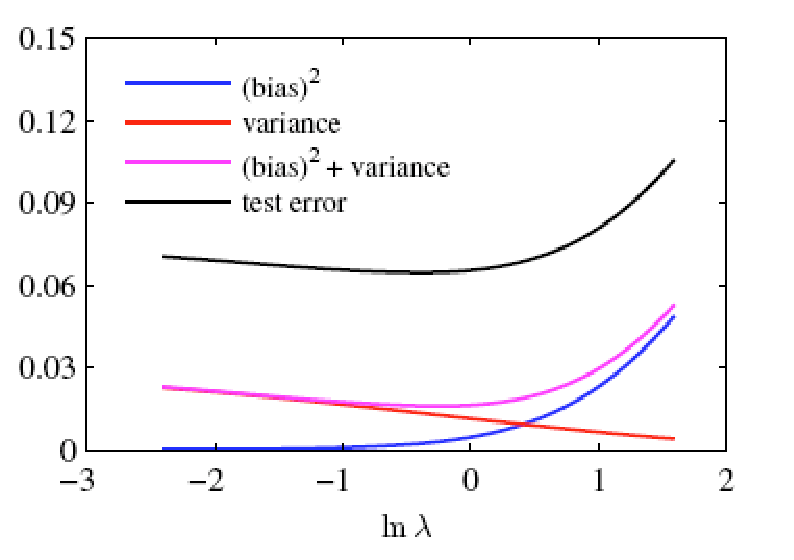
\includegraphics[width=.3\linewidth]{figure/fig17.pdf}}

\begin{itemize}
    \item The bias reflects the error introduced by approximating a real-life problem with a simplified model. As $\lambda$ increases (making the model simpler), bias increases.
    \item The variance reflects the sensitivity of the model to the specificities of the training set. As $\lambda$ increases, the model becomes less sensitive, and variance decreases.
\end{itemize}

The total error is the sum of $(\text{bias})^2$ and variance. The optimal value of $\lambda$ is located at the minimum of this sum, representing the point where the model is complex enough to capture the signal but simple enough to ignore the noise.
\end{myexample}



\subsection*{Probabilistic model for regression}
To move beyond simple function fitting and account for the inherent uncertainties in data, we now shift our focus to a probabilistic framework. This transition allows us to treat the relationship between inputs and targets not as a rigid deterministic rule, but as a class of joint probability distributions. By doing so, we can select the most probable model given our training data.

%\subsection*{The Gaussian Noise Model}
\medskip
We begin by defining the class of joint distributions $p(\x, t) = p_M(\x)p_C(t|\x)$. In this context, we assume the distribution of inputs $p_M(\x)$ is uniform, which allows us to concentrate entirely on the conditional distribution $p_C(t|\x)$. 

The core assumption of our model is that the observed target $t$, for a given input $\x$, is normally distributed around the value predicted by our hypothesis $h(\x; \ow)$. This variability is captured by a Gaussian distribution with a variance $\sigma^2$ or, as it is often expressed in Bayesian literature, a \alert{precision} $\beta$ (where $\beta = 1/\sigma^2$). Mathematically, this is expressed as:
\begin{myequation}
p(t|\x; \ow, \beta) = \mathcal{N}(t | h(\x; \ow), \beta^{-1})
\end{myequation}

This definition implies that our model $h(\x; \ow)$ represents the mean of the distribution, while $\beta$ represents our certainty: a higher precision means the observed data points are expected to cluster tightly around the model's prediction.

\begin{center}

\includegraphics[width=10cm]{Figure1-16.pdf}
\end{center}


\subsection*{Maximum Likelihood Estimation (MLE)}

Having established a probabilistic model, we need a criterion to estimate the parameters $\ow$ and the noise precision $\beta$. In a frequentist approach, we use the \alert{Likelihood function}, which measures how well a specific set of parameters explains the observed training set $(\X, \t)$. Assuming the observations are independent and identically distributed (i.i.d.), the likelihood is the product of the individual probabilities:
\begin{myequation}
L(\ow, \beta | \X, \t) = p(\t | \X; \ow, \beta) = \prod_{i=1}^n \mathcal{N}(t_i | h(\x_i; \ow), \beta^{-1}) = \prod_{i=1}^n \frac{\sqrt{\beta}}{\sqrt{2\pi}} e^{-\frac{\beta}{2}r_i(\ow)^2}
\end{myequation}

To simplify the optimization, we maximize the \alert{Log-Likelihood} $l(\ow, \beta | \X, \t)$, as the logarithm is a monotonic function that turns the product into a more manageable sum:
\begin{myequation}
l(\ow, \beta | \X, \t) = \sum_{i=1}^n \log \mathcal{N}(t_i | h(\x_i; \ow), \beta^{-1})
\end{myequation}
By expanding the Gaussian definition and taking the log, we obtain:
\begin{myalign}
l(\ow, \beta | \X, \t) &= -\frac{\beta}{2} \sum_{i=1}^n r_i(\ow)^2 + \frac{n}{2} \log \beta + c
\end{myalign}
where $c$ is a constant independent of $\ow$ and $\beta$.

%\subsubsection*{Deriving $\ow_{ML}$ and $\beta_{ML}$}

The maximization of this objective reveals a deep connection between probability and geometry:
\begin{itemize}
    \item For the weights $\ow$, maximizing the log-likelihood is equivalent to maximizing $-\frac{1}{2} \sum r_i(\ow)^2$, which is exactly the same as \textbf{minimizing the sum of squared errors}. This proves that Least Squares is the optimal frequentist estimator under the assumption of Gaussian noise.
    \item For the precision $\beta$, by setting the derivative with respect to $\beta$ to zero:
    \begin{myequation}
    \frac{\partial l}{\partial \beta} = -\frac{1}{2} \sum_{i=1}^n r_i(\ow)^2 + \frac{n}{2\beta} = 0
    \end{myequation}
    We find that the maximum likelihood estimate for the noise variance is the average of the squared residuals:
    \begin{myequation}
    \beta_{ML}^{-1} = \frac{1}{n} \sum_{i=1}^n r_i(\ow)^2
    \end{myequation}
\end{itemize}

As a result of this estimation, we obtain a \alert{predictive distribution}. Instead of returning a single point estimate for a new input $\x$, the model now provides a full Gaussian density:
\begin{myequation}
p(t | \x; \ow_{ML}, \beta_{ML}) = \mathcal{N}(t | h(\x; \ow_{ML}), \beta_{ML}^{-1})
\end{myequation}

\subsection*{The Bayesian Approach and Conjugate Priors}

While MLE is powerful, it is strictly frequentist: it treats parameters as fixed, unknown constants and is highly susceptible to overfitting when the dataset is small. To introduce regularization within a probabilistic context, we move to the \alert{Bayesian framework}. Here, parameters $\ow$ are treated as random variables with their own probability distributions.

Before seeing the data, we assume a \alert{prior distribution} $p(\ow | \alpha)$. We typically choose a zero-mean Gaussian prior with a diagonal covariance matrix, governed by the hyperparameter $\alpha$:
\begin{myequation}
p(\ow | \alpha) = \mathcal{N}(\ow; \Zero, \alpha^{-1}\I) = \left(\frac{\alpha}{2\pi}\right)^{\frac{m}{2}} e^{-\frac{\alpha}{2}\ow^T\ow}
\end{myequation}

\begin{center}

\includegraphics[width=.3\linewidth]{Figure_1.pdf}
\end{center}


%\subsubsection*{The Posterior Distribution}

The choice of a Gaussian prior is strategically significant because the Gaussian is a \textbf{conjugate prior} for the mean of a Gaussian likelihood. This means that the resulting \alert{posterior distribution}—the distribution of parameters after observing the training data—will also be Gaussian. According to Bayes' rule:
\begin{myequation}
p(\ow | \X, \t; \alpha, \beta) \propto p(\t | \X, \ow; \beta) p(\ow | \alpha)
\end{myequation}

Given a general Gaussian prior $p(\ow) = \mathcal{N}(\ow; \Vbold{m}_0, \Sigma_0)$, the posterior is $p(\ow | \X, \t) = \mathcal{N}(\ow; \Vbold{m}_p, \Sigma_p)$ where:
\begin{myalign}
\Sigma_p &= (\Sigma_0^{-1} + \beta \oX^T \oX)^{-1} \\
\Vbold{m}_p &= \Sigma_p (\Sigma_0^{-1} \Vbold{m}_0 + \beta \oX^T \t)
\end{myalign}

In our specific case, with a zero-mean prior ($\Vbold{m}_0 = \Zero$) and precision $\alpha$ ($\Sigma_0^{-1} = \alpha\I$), the posterior parameters simplify to:
\begin{myalign}
\Sigma_p &= (\alpha\I + \beta\oX^T \oX)^{-1} \\
\Vbold{m}_p &= \beta \Sigma_p \oX^T \t
\end{myalign}

Observe that the mean of the posterior $\Vbold{m}_p$ is exactly the same as the solution for Ridge Regression. In the Bayesian view, regularization is not just an arbitrary penalty added to the loss function; it is the natural consequence of assuming that the parameters themselves follow a Gaussian distribution centered at zero. As $\alpha \to 0$ (meaning we have no prior information), the posterior mean $\Vbold{m}_p$ converges back to the Maximum Likelihood estimate $\ow_{ML}$.

\subsection*{Sequential Bayesian Learning}

A significant advantage of the Bayesian approach to linear regression is its inherent ability to process data incrementally. Unlike batch methods that require all data to be present simultaneously, Bayesian inference allows us to update our knowledge as new information arrives. 

%\subsection*{The Recursive Nature of Posterior Updates}

The core principle of sequential learning is that the posterior distribution obtained after observing a specific subset of data can serve as the prior distribution for the next phase of learning. This recursive update is a direct consequence of Bayes' Theorem. 

When we receive a sequence of independent training sets $\mathcal{T}_{1}, \ldots, \mathcal{T}_{n}$, we can update our beliefs about the parameter vector $\ow$ step-by-step. For the first dataset $\mathcal{T}_{1}$, the posterior is proportional to the product of the likelihood and the initial prior:
\begin{myalign}
p(\ow| \mathcal{T}_{1}) &\propto p(\mathcal{T}_{1}|\ow)p(\ow)
\end{myalign}
For any subsequent step $k$, the current posterior is updated using the new likelihood $p(\mathcal{T}_{k}|\ow)$ and the previous posterior, which now acts as the prior:
\begin{myalign}
p(\ow| \mathcal{T}_{1}, \ldots, \mathcal{T}_{k}) &\propto p(\mathcal{T}_{k}|\ow) p(\ow| \mathcal{T}_{1}, \ldots, \mathcal{T}_{k-1})
\end{myalign}
This chain of updates continues as more data is acquired:
\begin{myalign}
p(\ow| \mathcal{T}_{1},\ldots, \mathcal{T}_{n}) &\propto p(\mathcal{T}_{n}|\ow)p(\ow| \mathcal{T}_{1},\ldots, \mathcal{T}_{n-1})
\end{myalign}

This "online" learning capability is extremely valuable in scenarios where data is collected in a stream or where the dataset is too large to fit into memory all at once. Every new observation refines our distribution, typically narrowing the variance and shifting the mean toward the true underlying parameters.

%\subsection*{Illustrative Example: Linear Regression Parameter Space}
\begin{myexample}

To visualize this process, let us consider a practical example of a simple linear regression model with one input variable $x$ and one target variable $t$. The model is defined by two parameters: the slope $w_1$ and the intercept $b$ (which we will also refer to as $w_0$):
\begin{myequation}
h(x; b, w_{1}) = w_{1}x + b
\end{myequation}



%\subsubsection*{Experimental Setup}

The data for this example is generated from a "ground truth" linear function $y = a_0 + a_1x$, where $a_0 = -0.3$ and $a_1 = 0.5$. The input values $x$ are sampled uniformly from the interval $[-1, 1]$, and the targets are corrupted by adding zero-mean Gaussian noise with a standard deviation $\sigma = 0.2$.

Before observing any data, we must define our initial state of knowledge. We assume a bivariate Gaussian prior distribution $p(w_{1}, b)$ centered at the origin, reflecting our initial lack of a preferred direction or intercept:
\begin{myequation}
\Vmu = \Zero, \quad \VSigma = \sigma^{2}\I = 0.04\I
\end{myequation}


\textit{Initial State:} On the left, the prior distribution is a broad circle centered at $(0,0)$. On the right, 6 lines are sampled by drawing weights $(w_0, w_1)$ from this prior. These lines appear in random orientations because the prior is uninformative.
\centerline{\begin{tabular}{rcl}

\includegraphics[width=.3\textwidth]{blrpp1.pdf}&
 \hspace{2mm}&

\includegraphics[width=.3\textwidth]{blrds1.pdf}
\end{tabular}}
%\subsubsection*{Learning from a Single Observation}

Once we observe the first item $(x_{1}, t_{1})$, represented by a circle in the right-hand plot, our knowledge is updated. The likelihood of this single point "carves" a path through the parameter space.


\textit{First Update:} The posterior distribution $p(w_{0}, w_{1} | x_{1}, t_{1})$ (left) is no longer circular; it has been elongated into a stripe. This stripe represents all combinations of $b$ and $w_1$ that could reasonably explain the single observed point. Consequently, the sampled lines (right) now all pass relatively close to that first observation.

\centerline{\begin{tabular}{rcl}

\includegraphics[width=.3\textwidth]{blrpp2.pdf}&
 \hspace{2mm}&

\includegraphics[width=.3\textwidth]{blrpp2.pdf}
\end{tabular}}
%\subsubsection*{Incremental Refinement}

As we observe a second item $(x_{2}, t_{2})$, the posterior is updated again. The intersection of the "knowledge" from the first point and the "knowledge" from the second point further constrains the parameters.


\textit{Second Update:} The posterior (left) is now concentrated in the region where the requirements for both observed points are met. The sampled lines (right) are now much more restricted, as they must pass through the vicinity of both circles.

\centerline{\begin{tabular}{rcl}

\includegraphics[width=.3\textwidth]{blrpp3.pdf}&
 \hspace{2mm}&

\includegraphics[width=.3\textwidth]{blrds3.pdf}
\end{tabular}}
%\subsubsection*{Convergence to the True Model}

Finally, after observing a larger set of $n$ items, the cumulative effect of the likelihood terms dominates the initial prior.
%\section*{Mathematical Proof of Decreasing Posterior Variance}



\textit{Final State:}
\begin{itemize}
\item \textbf{Parameter Concentration:} As the number of observed items increases, the posterior distribution of $w_{0}$ and $w_{1}$ becomes highly concentrated. The variance decreases toward zero, and the distribution converges around the true parameter values $a_{0} = -0.3$ and $a_{1} = 0.5$. 
\item \textbf{Model Accuracy:} As a direct consequence, the lines sampled from this tight posterior are nearly indistinguishable from each other and are concentrated precisely around the true generating function $y = -0.3 + 0.5x$.
\end{itemize}
\centerline{\begin{tabular}{rcl}

\includegraphics[width=.3\textwidth]{blrpp4.pdf}&
 \hspace{2mm}&

\includegraphics[width=.3\textwidth]{blrds4.pdf}
\end{tabular}}

This visual evolution demonstrates how the Bayesian framework naturally handles the transition from high uncertainty (the broad prior) to high certainty (the sharp posterior) as evidence accumulates.
\end{myexample}

\medskip
To understand why our certainty increases with more data, we can examine the evolution of the posterior covariance matrix $\Sigma_n$ as we transition from $n$ to $n+1$ observations.

Recall the general form of the posterior covariance matrix for a Gaussian prior and likelihood:
\begin{myequation}
\Sigma_p^{-1} = \Sigma_0^{-1} + \beta \oX^T \oX
\end{myequation}
where $\Sigma_0^{-1}$ is the prior precision, $\beta$ is the noise precision of the data, and $\VPhi_n$ is the design matrix for $n$ observations.

When a new observation $(\x_{n+1}, t_{n+1})$ is acquired, the new design matrix $\oX_{n+1}$ is simply the previous matrix $\oX_n$ with an additional row $\ox_{n+1}^T$ appended. The product $\oX_{n+1}^T \oX_{n+1}$ can be decomposed as:
\begin{myequation}
\oX_{n+1}^T \oX_{n+1} = \oX_n^T \oX_n + \ox_{n+1}\ox_{n+1}^T
\end{myequation}

Substituting this into our update rule for the posterior precision $\Sigma_{n+1}^{-1}$, we get:
\begin{myequation}
\Sigma_{n+1}^{-1} = \Sigma_n^{-1} + \beta \ox_{n+1}\ox_{n+1}^T
\end{myequation}

The term $\ox_{n+1}\ox_{n+1}^T$ is a positive semi-definite matrix. This means that with every new observation, we are adding a non-negative amount of information to the precision matrix. Since the precision increases, the "size" of the covariance matrix $\Sigma$ (measured by its eigenvalues) must decrease.

%\subsection*{The Woodbury Identity and the Reduction of Variance}

To see how the actual variance decreases in a specific direction, we can use the \textbf{Sherman-Morrison formula} (a special case of the Woodbury matrix identity) to find the update for the covariance matrix itself:
\begin{myequation}
\Sigma_{n+1} = \left( \Sigma_n^{-1} + \beta \oX \oX^T \right)^{-1} = \Sigma_n - \frac{\Sigma_n \oX \oX^T \Sigma_n}{\beta^{-1} + \oX^T \Sigma_n \oX}
\end{myequation}
 From this expression, we can derive the change in variance:
\begin{myequation}
\Delta \Sigma = \Sigma_n - \Sigma_{n+1} = \frac{\Sigma_n \oX \oX^T \Sigma_n}{\beta^{-1} + \oX^Txx \Sigma_n \oX}
\end{myequation}

Because the denominator is a scalar sum of positive terms (the noise variance and the projected parameter variance) and the numerator is a quadratic form $\Vbold{v}\Vbold{v}^T$ (where $\Vbold{v} = \Sigma_n \Vphi$), the resulting matrix $\Delta \Sigma$ is \textbf{positive semi-definite}. 

This proves that $\Sigma_{n+1} \preceq \Sigma_n$ in the sense of the Loewner partial ordering. Geometrically, the "uncertainty ellipsoid" in the parameter space can only shrink or remain the same size as more data is observed; it can never expand. This is exactly what we observed in the sequential learning example, where the broad circular prior collapsed into a tiny, dense point.
This reduction in parameter variance is what ultimately leads to the narrowing of the uncertainty bands in the predictive distribution.

\subsubsection*{Maximum a Posteriori}

Once we have established the posterior distribution $p(\ow|\X, \t; \alpha, \beta)$, we face the task of selecting a representative set of parameters from this distribution to make predictions. In the Bayesian framework, the most natural single-point representative is the \alert{Maximum A Posteriori (MAP)} estimate, $\ow_{MAP}$. This vector represents the \alert{mode} of the posterior distribution—the point where the probability density is at its highest.

%\subsection*{Deriving the MAP Objective}

To find the MAP estimate, we seek the value of $\ow$ that maximizes the posterior probability. Mathematically, it is more convenient to work with the logarithm of the probability, as it simplifies the product of the likelihood and the prior into a sum. Using Bayes' rule, the log-posterior is expressed as:
\begin{myequation}
\log p(\ow|\X, \t; \alpha, \beta) = \log p(\t | \X, \ow, \beta) + \log p(\ow; \alpha) - \log p(\t | \X; \beta)
\end{myequation}
Since the term $p(\t | \X; \beta)$ (the evidence) does not depend on $\ow$, it acts as a constant during the optimization process. Therefore, the maximization simplifies to:
\begin{myequation}
\ow_{MAP} = \argmax{\ow} \left( \log p(\t | \X, \ow; \beta) + \log p(\ow ; \alpha) \right)
\end{myequation}
By simply changing the sign, we can reformulate this as a minimization problem, which is common in optimization literature:
\begin{myequation}
\ow_{MAP} = \argmin{\ow} \left( -\log p(\t|\X,\ow;\beta) - \log p(\ow; \alpha) \right)
\end{myequation}

%\subsection*{Connecting Probability to Regularized Least Squares}

To understand what this means in the case of gaussian model for regression considered here, we expand the terms using our Gaussian assumptions for both the likelihood and the prior. For the likelihood, we have:
\begin{myequation}
\log p(\t|\X, \ow; \beta) = \sum_{i=1}^n \left( \frac{1}{2} \log \frac{\beta}{2\pi} - \frac{\beta}{2} r_i(\ow)^2 \right) = \frac{n}{2} \log \frac{\beta}{2\pi} - \frac{\beta}{2} \sum_{i=1}^n r_i(\ow)^2
\end{myequation}
Similarly, for the Gaussian prior on the $d+1$ parameters (including the bias $\overline{w}_0$):
\begin{myequation}
\log p(\ow; \alpha) = \sum_{j=0}^d \left( \frac{1}{2} \log \frac{\alpha}{2\pi} - \frac{\alpha}{2} \overline{w}_j^2 \right) = \frac{d+1}{2} \log \frac{\alpha}{2\pi} - \frac{\alpha}{2} \sum_{j=0}^d \overline{w}_j^2
\end{myequation}

By combining these and dropping the constants that do not involve $\ow$, we find that maximizing the posterior probability is equivalent to minimizing the following expression:
\begin{myequation}
\frac{\beta}{2} \sum_{i=1}^n r_i(\ow)^2 + \frac{\alpha}{2} \sum_{j=0}^d \overline{w}_j^2 \propto \frac{1}{2} \sum_{i=1}^n r_i(\w)^2 + \frac{\alpha}{2\beta} \sum_{j=0}^d \overline{w}_j^2
\end{myequation}

This result is significant because it provides a probabilistic justification for \alert{Ridge Regression}. The ratio of the two precision hyperparameters, $\lambda = \frac{\alpha}{\beta}$, corresponds exactly to the regularization hyperparameter $\lambda$ we introduced earlier. We can now see that regularization is not just a heuristic to prevent overfitting; it is the direct consequence of assuming a Gaussian prior on the model parameters. 



%\subsection*{The Predictive Distribution in the MAP Context}

With the MAP estimate in hand, we can define the \alert{predictive distribution} for a target value $t$ given a new input $\x$. Just as in the Maximum Likelihood (ML) framework, the result is a Gaussian distribution centered at the model's prediction:
\begin{myequation}
p(t|\x, \ow_{MAP}; \beta_{MAP}) = \mathcal{N}(t|h(\x;\ow_{MAP}),\beta_{MAP}^{-1}) = \sqrt{\frac{\beta_{MAP}}{2\pi}}e^{-\frac{\beta_{MAP}}{2}\left(h(\x,\ow_{MAP})-t\right)^2}
\end{myequation} 
In this context, it can be shown that the MAP estimate for the precision, $\beta_{MAP}$, is equivalent to the $\beta_{ML}$ value derived previously, representing the noise variance of the training data.

While the MAP estimate provides a more robust prediction than ML by incorporating prior knowledge, it still only uses a single point estimate of $\ow$. A fully Bayesian approach would instead integrate over all possible values of $\ow$ to account for parameter uncertainty.



\subsection*{Approaches to prediction in linear regression}

\subsection*{Classical}
A value $\ow_{LS}$ for $\ow$ is learned through a point estimate, performed by minimizing a quadratic cost function, or equivalently by maximizing likelihood (ML) under the hypothesis of gaussian noise; regularization can be applied to modify the cost function to limit overfitting. 

Given any $\x$, the obtained value $\ow_{LS}$ is used to predict the corresponding $t$ as $t=\ox^T\ow_{LS}=\x^T\w_{LS}+b_{LS}$.



\subsection*{Bayesian point estimation}
The posterior distribution $p(\ow|\X,\t; \alpha,\beta)$  is derived and a point estimate is performed from it, computing the mode $\ow_{MAP}$ of the distribution (MAP). 

This is equivalent to the classical approach, as $\ow_{MAP}$ corresponds to $\ow_{LS}$ if $\lambda=\textstyle\frac{\alpha}{\beta}$. The prediction, for an element $\x$, is a gaussian distribution  $\mathcal{N}(t|\ox^T\ow_{MAP}, \beta)$ for $t$, with mean $\ox^{T}\ow_{MAP}=\x^T\w_{MAP}+b_{MAP}$ and variance $\beta^{-1}$.

The distribution is not derived directly from the posterior  $p(\ow|\X,\t;\alpha,\beta)$: it is built, instead, as a gaussian with mean depending from the expectation of the posterior, and variance given by the assumed noise.

\subsection*{Fully bayesian}
The real interest is not in estimating $\ow$ or its distribution $p(\ow|\X,\t;\alpha,\beta)$, but in deriving the \alert{predictive distribution} $p(t|\x, \X, \t)$, which expresses our uncertainty about the target $t$ for a new input $\x$, given the entire training history. This can be done computing the expectation of the probability $p(t|\x, \ow;\beta)$ predicted by a model instance wrt  model instance distribution $p(\ow|\X,\t;\alpha,\beta)$, that is also by marginalization wrt to  $\w$
\begin{myequation}
p(t|\x, \t,\X;\alpha,\beta)=\int p(t|\x, \ow;\beta)p(\ow|\t,\X;\alpha,\beta)d\ow
\end{myequation}

This integral represents a convolution of two Gaussian distributions:
\begin{itemize}
    \item $p(t|\x, \ow; \beta)$, the \alert{likelihood} of a target given a specific $\ow$.
    \item $p(\ow|\X, \t; \alpha, \beta)$, the \alert{posterior distribution} of the weights we derived previously.
\end{itemize}

%\item since $p(\w|\t,\VPhi,\alpha,\beta)$
The distribution $p(t|\x,\ow;\beta)$ is assumed gaussian, and $p(\ow|\X, \t, ;\alpha,\beta)$ is gaussian by the assumption that the likelihood $p(\t|\X,\ow; \beta)$ and the prior $p(\ow;\alpha)$ are gaussian themselves and by their being conjugate
\begin{myalign}
%p(y|\x, \t,\VPhi,\alpha,\beta)&=\mathcal{N}(y|\x^{T}\w_{MAP}, \beta)\\
p(t|\x, \w;\beta)&=\mathcal{N}(t|\ow^T\ox, \beta)\\
p(\ow|\X, \t;\alpha,\beta)&=\mathcal{N}(\ow;\beta\Sigma\oX^{T}\t, \Sigma)
\end{myalign}

where $\Sigma=(\alpha\I+\beta\oX^{T}\oX)^{-1}$ is a $(d+1)\times (d+1)$ matrix.


Under such hypothesis, the predictive distribution is gaussian
\begin{myequation}
p(t|\x, \X,\t;\alpha,\beta)=\mathcal{N}(t;m(\x), \sigma^2(\x))
\end{myequation}
%$
%\gaussiandistr{y|\x, \y,\VPhi,\alpha,\sigma^{2}}{\overline{\Vmu}}{\overline{\VSigma}}
%$
with mean 
\begin{myequation}
m(\x)=\beta\ox^{T}\Sigma\oX^{T}\t
\end{myequation}
and variance
\begin{myequation}
\sigma^{2}(\x)=\frac{1}{\beta}+\ox^{T}\Sigma\ox
\end{myequation}
%e media
%\begin{myequation}
%\overline{\mu}(\x)=\x^{T}\sigma^{-2}\VSigma\VPhi^{T}\y=\sigma^{-2}\x^{T}\VSigma\VPhi^{T}\y
%\end{myequation}

The predictive variance $\sigma^2(\x)$ is composed of two distinct parts that highlight the power of the Bayesian method:
\begin{enumerate}
    \item $\frac{1}{\beta}$: This is the \alert{intrinsic noise} in the data (aleatoric uncertainty). It represents the fundamental limit of predictability; even if we knew the true parameters perfectly, the noise $\varepsilon$ would still exist.
    \item $\ox^{T}\Sigma\ox$: This is the \alert{parameter uncertainty} (epistemic uncertainty). It represents our lack of knowledge about the "true" $\ow$. 
\end{enumerate}


\begin{myexample}
Example: evolution of the Bayesian Predictive Distribution

\medskip
In this example, we examine how the Bayesian framework's understanding of the function $f(x) = \sin(2\pi x)$ evolves as it encounters increasing amounts of data. We utilize a model consisting of $m=9$ Gaussian basis functions. This relatively high degree of complexity would typically lead to severe overfitting in a frequentist setting, but here we observe how the Bayesian predictive distribution manages uncertainty.

%\subsection*{Structure of the Visualization}

The following figures illustrate the model's state after observing training sets of $n=1, 2, 4,$ and $25$ items respectively. For each stage of the experiment, the visualization is divided into two parts:

\begin{itemize}
    \item Left (Predictive Distribution): The blue circles represent the items in the training set, which are sampled uniformly from the input space with added Gaussian noise. The \textbf{red line} represents the expectation (the mean) of the predictive distribution $p(t|x, \X, \t)$, effectively our current best guess for the function. The \textbf{pink shaded region} represents the variance, specifically showing one standard deviation from the mean. This captures the model's total uncertainty, including both the noise in the data and the uncertainty regarding the parameters.
    
    \item Right (Posterior Samples): Again, we see the training items, but here they are overlaid with \textbf{5 possible curves}. Each curve is generated by taking a random sample of weights $\ow$ from the current posterior distribution $p(\ow|\X, \t; \alpha, \beta)$. This provides a qualitative sense of the "candidate functions" that the model still considers plausible.
\end{itemize}

%\subsection*{Observation of the Learning Process}

As we increase the number of observations $n$, we can follow the transition from ignorance to specialized knowledge.

\begin{description}
\item[The Case of $n=1$.]
With only a single data point, the model has almost no information about the frequency or amplitude of the sine wave.

\centerline{
\includegraphics[width=.6\textwidth]{preddistr1.pdf}}


On the left, the predictive mean is essentially forced through the single point but remains nearly flat elsewhere. The pink shaded region is extremely wide, indicating high uncertainty across the entire domain. On the right, the 5 sampled curves are wildly different from each other, showing that many different functions (sloping up, sloping down, or staying flat) are equally probable given only one point.

\item[The Case of $n=2$.]
Adding just one more point begins to constrain the possible orientations of the function.

\centerline{
\includegraphics[width=.6\textwidth]{preddistr2.pdf}}

As we see, the expectation (red line) now attempts to connect the two points. However, the variance (pink shade) is still quite large, particularly in the regions far from these two observations. The sampled curves on the right start to align slightly but still show a vast range of possible shapes.

\item[The Case of $n=4$.]
With four points, the characteristic "S" shape of the sine wave begins to emerge.

\centerline{
\includegraphics[width=.6\textwidth]{preddistr4.pdf}}

An important observation here is that the pink uncertainty band is not uniform. It "pinches" or narrows at the locations of the training items and widens in the gaps between them. This shows the model's confidence is localized; it knows the function better where it has seen data. The sampled curves on the right are now becoming more consistent, all sharing the same general oscillation.

\item[The Case of $n=25$.]
With twenty-five points, the model has gathered sufficient evidence to largely resolve the underlying signal.

\centerline{
\includegraphics[width=.6\textwidth]{preddistr25.pdf}}

At $n=25$, the predictive mean (red line) is an excellent approximation of $f(x) = \sin(2\pi x)$. Most importantly, the variance (pink shade) has collapsed significantly and is now nearly uniform across the domain. The 5 sampled curves on the right are now so similar that they are almost indistinguishable, indicating that the posterior distribution has become very peaky (low variance) around the optimal weights.
\end{description}
In this specific example, we see the Bayesian power to provide not just a curve, but a "margin of error" that naturally shrinks as the training set grows.
\end{myexample}

%\section*{The Mathematics of Predictive Uncertainty}

The predictive distribution $p(t|\x, \t)$ provides a Gaussian measure of the target $t$ for a new input $\x$. Its variance, $\sigma^2_n(\x)$, defines the "pink shade" observed in our previous plots. As observed before, this variance is the sum of two distinct components:

\begin{myequation}
\sigma^2_n(\x) = \underbrace{\frac{1}{\beta}}_{\text{Noise}} + \underbrace{\ox^{T}\Sigma\ox}_{\text{Model Uncertainty}}
\end{myequation}



The term $\ox^{T}\Sigma\ox$ is a quadratic form that measures how much the current parameter uncertainty "projects" onto the prediction at point $\x$. 

As we saw in the sequential learning example, the precision matrix $\Sigma\ox^{-1}$ is updated by adding the outer products of the basis vectors of the training points:
\begin{myequation}
\Sigma_n^{-1} = \Sigma_0^{-1} + \beta \sum_{i=1}^n \ox\ox^T
\end{myequation}

When we evaluate the model at a new point $\x$ that is very close to a training point $\x_i$, the vector $\ox$ becomes highly aligned with the direction in which we have already gained significant information (the eigenvectors of $\Sigma^{-1}$ with large eigenvalues). Mathematically, this causes the quadratic form $\ox^{T}\Sigma\ox$ to decrease significantly.

Conversely, in "data-void" regions where $\x$ is far from any $\x_i$, the vector $\ox$ points in a direction where the precision matrix has not been "strengthened" by the summation. Consequently, the term remains large, resulting in the wider pink bands between the blue training points.

The model is effectively saying: "I have seen samples in this neighborhood, so my parameters are well-constrained for this specific type of input; however, for inputs I haven't seen, my parameter uncertainty remains high." This is why, in the $n=25$ plot, the pink shade is almost uniform: the basis functions are sufficiently 'covered' by data points across the entire domain.

\subsection*{Fully bayesian regression and hyperparameter marginalization}
In a fully Bayesian treatment, we should ideally marginalize over the hyperparameters $\alpha$ and $\beta$ by defining hyperpriors.
\begin{myequation}
p(t|\x, \X, \t)=\int p(t|\x, \ow;\beta)p(\ow|\X, \t; \alpha,\beta)p(\alpha,\beta|\X, \t)\; d\ow\; d\alpha\; d\beta
\end{myequation}
where, as seen before,
\begin{itemize}
\item $p(t|\x, \ow,\beta)=\mathcal{N} (t; \ow^T\ox, \beta)$
\item $p(\ow|\X, \t, \alpha,\beta)=\mathcal{N}(\ow;\Vbold{m}_N,\Sigma)$, with $\Sigma=(\alpha\I+\beta\oX^T\oX)^{-1}$ e $\Vbold{m}_N=\beta\Sigma\oX^T\t$
\end{itemize}
this marginalization wrt $\w,\alpha,\beta$ is analytically intractable:
we may however consider approximation methods. 

% , that we do not introduce here.% where point estimation is applied to derive hyper-parameter values by maximizing the posterior distribution $p(\alpha,\beta|\t,\VPhi)$



\subsubsection*{Approximating the Hierarchical Bayesian Integral}

To finalize our discussion on the Bayesian treatment of linear regression, we address the situation where the marginalization over hyperparameters becomes a necessity. In a fully hierarchical Bayesian model, we do not simply select fixed values for $\alpha$ and $\beta$. Instead, we ideally integrate them out to ensure that our uncertainty about the model's complexity and noise levels is reflected in our final predictions.

The goal is to compute the \alert{predictive distribution} by accounting for the uncertainty in both the parameters $\ow$ and the hyperparameters $\alpha, \beta$:

\begin{myequation}
p(t|\x, \X, \t) = \int p(t|\x, \ow; \beta) p(\ow|\X, \t; \alpha, \beta) p(\alpha, \beta|\X, \t) \, d\ow \, d\alpha \, d\beta
\end{myequation}

In this expression, we recognize the following components:
\begin{itemize}
    \item The Likelihood $p(t|\x, \ow, \beta) = \mathcal{N}(t; \ow^T\ox), \beta^{-1})$, defining the distribution of the target around the model's prediction.
    \item The Weight Posterior $p(\ow|\X, \t, \alpha, \beta) = \mathcal{N}(\ow; \Vbold{m}_N, \Sigma)$, where $\Sigma = (\alpha\I + \beta\oX^T\oX)^{-1}$ and $\Vbold{m}_N = \beta\Sigma\oX^T\t$.
    \item The Hyperparameter Posterior: $p(\alpha, \beta | \X, \t)$, representing our updated belief about regularization and noise after observing the training data.
\end{itemize}

The non-linear dependence of the weight posterior (specifically the mean $\Vbold{m}_N$ and covariance $\Sigma$) on the hyperparameters prevents the evaluation of the integral in a closed form. To deal with this, we employ various approximation methods can be employed.

\begin{description}
\item[The Laplace Approximation.]
The Laplace approximation is a deterministic method used to approximate a complicated, non-Gaussian distribution with a Gaussian one. It works by finding the \alert{mode} of the distribution (the MAP estimate) and performing a second-order Taylor expansion of the log-probability around that mode.


Mathematically, if we have a distribution $p(\Vbold{z}) = f(\Vbold{z})/Z$, we find the mode $\Vbold{z}_0$ and approximate the log-density as:
\begin{myequation}
\ln f(\Vbold{z}) \approx \ln f(\Vbold{z}_0) - \frac{1}{2}(\Vbold{z} - \Vbold{z}_0)^T \Vbold{A} (\Vbold{z} - \Vbold{z}_0)
\end{myequation}
where $\Vbold{A}$ is the \alert{Hessian matrix} (the matrix of second derivatives) of the negative log-probability. This effectively replaces the intractable hyperparameter posterior with a localized Gaussian, making the subsequent integration more manageable.

\item[Variational Inference (VI).]
Variational methods cast the inference problem as an optimization task rather than an integration task. We define a family of simpler distributions $q(\ow, \alpha, \beta)$ - often assuming they are independent, a technique known as the \textit{mean-field approximation} - and minimize the \alert{Kullback-Leibler (KL) divergence} between this proxy and the true, intractable posterior.



\item[Markov Chain Monte Carlo (MCMC).]
MCMC is a stochastic approach that bypasses the need for analytical integration entirely. By constructing a Markov chain that has the posterior $p(\ow, \alpha, \beta | \X, \t)$ as its equilibrium distribution, we can draw a series of samples $\{\ow^{(l)}, \alpha^{(l)}, \beta^{(l)}\}_{l=1}^L$. The predictive distribution is then approximated by the empirical average:

\begin{myequation}
p(t|\x, \X, \t) \approx \frac{1}{L} \sum_{l=1}^L p(t|\x, \ow^{(l)}, \beta^{(l)})
\end{myequation}

As the number of samples $L \to \infty$, this numerical approximation converges to the true value of the integral. While computationally intensive, it is the most flexible method for complex hierarchical models.

The choice between these methods depends on the size of the dataset and the required precision. In many linear regression contexts, the \alert{Evidence Framework} described below (which provides a point-estimate) is sufficient, but for highly non-linear or safety-critical applications, MCMC or Variational methods are preferred to ensure the full breadth of uncertainty is captured.

\medskip
\noindent Would you like me to demonstrate how \textbf{Gibbs Sampling}—a specific MCMC algorithm—would be implemented to sample from the posterior of $\ow$, $\alpha$, and $\beta$ in this model?
\end{description}

\subsection*{The Evidence Framework (Empirical Bayes)}

Up to this point, we have treated the hyperparameters $\alpha$ and $\beta$ as quantities that must be chosen externally, either by manual tuning or by computationally expensive procedures such as cross-validation. While these approaches can work in practice, they are conceptually unsatisfactory: they separate model training from hyperparameter selection and require additional data or repeated training cycles.

A more principled and elegant solution is provided by the \alert{evidence framework}, also known as \alert{Empirical Bayes}. The key idea is to treat $\alpha$ and $\beta$ not as arbitrary tuning parameters, but as quantities that can be inferred directly from the data in a probabilistically consistent manner.

Rather than selecting $\alpha$ and $\beta$ by hand, we choose the values that maximize the \alert{marginal likelihood} $p(\t|\alpha, \beta)$, commonly called the \alert{evidence}. This quantity measures how well the model, with given hyperparameters, explains the observed data after integrating out the model parameters $\ow$.

Formally, the evidence is defined as
\begin{myequation}
p(\t|\alpha, \beta) = \int p(\t|\ow, \beta)\, p(\ow|\alpha)\, d\ow .
\end{myequation}

This integral expresses a crucial Bayesian idea: instead of conditioning on a single parameter vector $\ow$, we average over all possible parameter values, weighted by their prior probability. In this sense, the evidence evaluates how plausible the data are under the entire model class defined by $\alpha$ and $\beta$, rather than under one specific fitted model.

\medskip
Because both the likelihood $p(\t|\ow,\beta)$ and the prior $p(\ow|\alpha)$ are Gaussian, this integral can be solved analytically. Taking the logarithm of the result leads to the \alert{log-evidence}:

\begin{myequation}
\log p(\t|\alpha, \beta)
= \frac{m}{2}\log \alpha
+ \frac{n}{2}\log \beta
- E(\Vbold{m}_p)
- \frac{1}{2}\log |\Vbold{A}|
- \frac{n}{2}\log(2\pi).
\end{myequation}

This expression contains several competing terms. The first two favor large values of $\alpha$ and $\beta$, while the remaining terms penalize overly complex or poorly fitting models. Maximizing the log-evidence therefore implements an automatic trade-off between data fit and model complexity.

\medskip
Two central quantities appear in this formula:

\begin{itemize}
    \item $\Vbold{A} = \Sigma^{-1} = \alpha\I + \beta\oX^T\oX$ is the \textbf{Hessian matrix} of the error function. It is the inverse of the posterior covariance matrix and quantifies the curvature of the log-posterior around its maximum. Intuitively, a larger $\Vbold{A}$ means a sharper, more concentrated posterior, indicating greater certainty about the parameter values.
    
    \item $\displaystyle E(\Vbold{m}_p)
    = \frac{\beta}{2}\|\t - \oX\Vbold{m}_p\|^2
    + \frac{\alpha}{2}\Vbold{m}_p^T\Vbold{m}_p$
    is the total regularized error evaluated at the posterior mean $\Vbold{m}_p$. The first term measures how well the model fits the data (residual error), while the second term penalizes large weights, enforcing smoothness and preventing overfitting.
\end{itemize}

\medskip
\bigskip
\noindent
\textbf{From the Hessian to the Effective Number of Parameters}

To determine the optimal hyperparameters, we maximize the log-evidence with respect to $\alpha$ and $\beta$. In doing so, a fundamental concept naturally emerges: the \alert{effective number of parameters}, denoted by $\gamma$.

The total precision of the posterior is governed by the Hessian matrix
\[
\Vbold{A} = \alpha\I + \beta\oX^T\oX.
\]
The term $\alpha\I$ represents the contribution of the prior, while $\beta\oX^T\oX$ encodes the information coming from the data. To understand their relative influence, we examine the eigenvalues $\eta_i$ of the data-dependent matrix $\beta\oX^T\oX$.

For each direction $i$ in parameter space, we define the ratio

\begin{myequation}
\lambda_i = \frac{\eta_i}{\alpha + \eta_i}.
\end{myequation}

This quantity behaves like a soft switch that tells us whether a parameter is mainly controlled by the data or by the prior.

\begin{itemize}
    \item \textbf{Data Dominance} ($\eta_i \gg \alpha$):  
    When the data provide strong information in direction $i$, the ratio $\lambda_i$ approaches 1. In this case, the prior has little influence, and the parameter is effectively determined by the data.

    \item \textbf{Prior Dominance} ($\eta_i \ll \alpha$):  
    When the data are weak or noisy in direction $i$, the ratio $\lambda_i$ approaches 0. Here, the prior dominates and effectively shrinks the corresponding parameter toward zero.
\end{itemize}

\medskip
The total effective number of parameters is then defined as the sum of these contributions across all $m$ dimensions:

\[
\gamma = \sum_{i=1}^m \frac{\eta_i}{\alpha + \eta_i}.
\]

This quantity has a clear interpretation: it counts how many independent directions in parameter space are truly informed by the data.

\begin{itemize}
    \item If $\gamma \approx m$, the dataset contains enough information to determine nearly all parameters, and regularization plays only a minor role.
    \item If $\gamma \ll m$, most parameters are constrained by the prior, meaning that the model is effectively using far fewer degrees of freedom than its nominal dimension.
\end{itemize}

\medskip
A useful intuition is given by the spring analogy. Imagine each weight as attached to two springs: one pulling toward zero (the prior, stiffness $\alpha$) and one pulling toward the data-driven estimate (stiffness $\eta_i$). If the data spring is much stronger, the weight moves toward the data; if the prior spring dominates, the weight remains near zero.

The quantity $\gamma$ tells us, in aggregate, how many weights have been significantly pulled away from zero by the data. This provides the conceptual foundation for automatically adapting model complexity using the Evidence Framework.

\bigskip
\subsubsection*{Estimation of the Optimal $\alpha$ and $\beta$}

Setting the derivatives of the log-evidence with respect to $\alpha$ and $\beta$ to zero leads to two re-estimation formulas.

\begin{itemize}
    \item The optimal $\alpha$ is inversely related to the average squared magnitude of the effective weights:

    \begin{myequation}
    \alpha = \frac{\gamma}{\Vbold{m}_p^T\Vbold{m}_p}.
    \end{myequation}

    This means that if the posterior weights are large, we reduce $\alpha$ (weaker regularization), whereas if they are small, we increase $\alpha$ to prevent overfitting.

    \item The optimal $\beta$ is determined by the residual variance, corrected for the effective degrees of freedom used by the model:

    \begin{myequation}
    \frac{1}{\beta}
    = \frac{1}{n - \gamma}
    \sum_{i=1}^n (t_i - \Vbold{m}_p^T \ox_i)^2.
    \end{myequation}

    The term $n-\gamma$ plays the role of an effective sample size, accounting for the fact that $\gamma$ parameters have been used to explain the data.
\end{itemize}

\medskip
Since both $\Vbold{m}_p$ and $\gamma$ depend on $\alpha$ and $\beta$, these equations must be solved iteratively. The procedure is:

\begin{enumerate}
    \item Initialize $\alpha$ and $\beta$ to reasonable starting values.
    \item Compute the posterior mean $\Vbold{m}_p$ and the effective number of parameters $\gamma$.
    \item Update $\alpha$ and $\beta$ using the formulas above.
    \item Repeat until convergence.
\end{enumerate}

\medskip
This iterative scheme typically converges quickly and provides a fully automated way to balance model complexity and data fit.

\medskip


The Evidence Framework implements an automatic form of complexity control. If the data are noisy (small $\beta$), the evidence is maximized by increasing $\alpha$, which shrinks the weights toward zero. If the data are clean and informative, $\gamma$ approaches $m$, allowing the model to use its full expressive power.

The major advantage is that this procedure relies solely on the training data, eliminating the need for a separate validation set or expensive cross-validation. In this sense, Empirical Bayes provides a self-consistent and computationally efficient method for model selection within a Bayesian framework.




%
%\clearpage
%\pagestyle{empty}
%\end{document}